\documentclass{article}
\usepackage{amsmath}
\usepackage{mathtools}
\usepackage{gensymb}
\usepackage[a4paper,inner=1.5cm,outer=1.5cm,top=2cm,bottom=0.5cm]{geometry} 
\usepackage{xcolor}                    
\usepackage{tikz}                           
\usepackage{multicol}
\usepackage{pgfplots}
\usetikzlibrary{calc}
\usetikzlibrary{intersections}
\usetikzlibrary{intersections,calc,angles,quotes}
\usetikzlibrary{shapes,arrows,positioning,decorations.pathreplacing,calc}
\usetikzlibrary{calc,angles,positioning,intersections,quotes,decorations.markings}
\usepackage{tkz-euclide}
\usetikzlibrary{backgrounds}
\usetikzlibrary{calc,through}
\usetikzlibrary{angles}
\usetikzlibrary{fadings}
\usetikzlibrary{shapes.geometric}
\usetikzlibrary{shapes.symbols}
\usepackage{draftwatermark}
\usepackage{mathptmx}

\SetWatermarkText{\textcolor{black!30}{Mathema Shukur}}
\SetWatermarkFontSize{2 cm}
\usepackage[utf8]{inputenc}
\usepackage{fontspec}

\setmainfont{[Kalpurush.ttf]}
\newfontface{\en}{[Arial.ttf]} %%this is optional, if you want to use a secondary font. Any english font is supported
\newlength\Radius
\setlength\Radius{4cm}
\begin{document} 
	\Large
	\textcolor{red}{Welcome To} 
	\\
	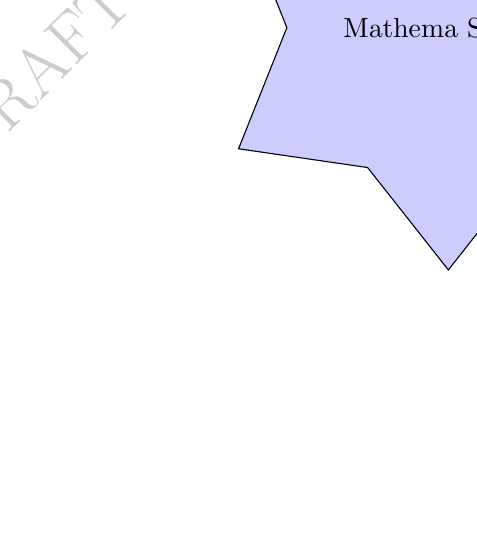
\begin{tikzpicture}
		\tikz \node [fill=blue!20,star,star points=6,draw] {Mathema Shukur };
	\end{tikzpicture}
	\\
	যাদের জন্যে প্রযোজ্যঃ  	\textcolor{magenta}{একাদশ ও দ্বাদশ শ্রেণীর শিক্ষার্থী} \\
	বিষয়ঃ \textcolor{magenta}{উচ্চতর গণিত ১ম পত্র} \\
	অধ্যায়ঃ \textcolor{magenta}{৩-সরলরেখা}\\ 
	Subtopicঃ  \textcolor{magenta}{  সরলরেখার বিভিন্ন আকারের সমীকরণ নির্ণয় করা   }\\
	\\
	\textcolor{blue}{(1)	ঢাল বিন্দু আকার Point slope form}\\
	\\
	$(y-y_1)=m(x-x_1)$\\
	\\
	\textcolor{red} {(2)  দুই বিন্দু আকার 	Two point form}\\
	\\
	$y-y_1=\left(\frac{y_1-y_2}{x_1-x_2}\right)(x-x_1)$\\
	\\
	\textcolor{green}{ (3) ঢাল খণ্ডন আকার 	Slope intercept form}\\
	\\
	$y=mx+c$\\
	\\
	\textcolor{cyan}{ (4) দ্বি খণ্ডন আকার  Two	Intercept form}\\
	\\
	$\frac{x}{a}+\frac{y}{b}=1$\\
	\\
	\\
	\textcolor{purple}{ (5) লম্ব  আকার  Normal form}\\
	\\
	মূল বিন্দু হতে কোনো সরলরেখার উপর অঙ্কিত লম্বের দৈর্ঘ্য $p$ এবং লম্বটি $x-$ অক্ষের ধনাত্মক দিকের সাথে $\alpha$ কোণ উৎপন্ন করলে, রেখাটির সমীকরণ নির্ণয় কর \\ 
	\\
	$x\cos \alpha +y\sin \alpha=p$\\
	\\
	\\
	\textcolor{olive}{ (6) সাধারণ/ আদর্শ  আকার  General form}\\
	\\
		$ax+by+c=0$\\
		\\
		দুই চলকের $(x,y)$ একঘাত (power 1) সমীকরণ সরলরেখার সাধারণ সমীকরণ প্রকাশ করে। এখানে $x$ এর ঘাত শুধু  মাত্র $1$ হবে  এবং $y$ এর ঘাত শুধুমাত্র $1$ হবে । এর ব্যতিক্রম হলে সমীকরণটি সরলরেখা নির্দেশ করবে না। \\
		\\ 
		যেমনঃ $ax^2+by=0$ এবং  $ax+by^3+2=0$ বক্র রেখা \\ 
		\\
	নিচের সমীকরণগুলিকে সাধারণ আকারে প্রকাশ কর\\
	\\
	$(1)\,\,y=\frac{3}{5}x+2$\\
	\\
	$(2)\,\,y-3=4(x+2)$\\
	\\ 
	$(3)\,\,\frac{x}{3}+\frac{y}{2}=1$\\
	\\ 
	\begin{align*}
	(1)\,\,y&=\frac{3}{5}x+2\\
	\\
	5y&=3x+10\\
	\\
	3x-5y+10&=0
	\end{align*}
\\
\begin{align*}
(2)\,\,y-3&=4(x+2)\\
\\
y-3&=4x+8\\
\\
4x-y+11&=0
\end{align*}
\\
\begin{align*}
(3)\,\,\frac{x}{3}+\frac{y}{2}&=1\\
\\
2x+3y&=6
\end{align*}
\\
সরলরেখার সাধারণ সমীকরণ	$ax+by+c=0$ এর আলোকে নিচের শর্তগুলি ব্যাখ্যা কর \\ 
	\begin{align*}
		(1)\,\,\,& a=0,\quad b\ne 0,\quad c\ne 0\\
		\\
		(2)\,\,\, & a=0,\quad b\ne 0,\quad c=0\\
		\\
		(3)\,\,\,& a\ne 0,\quad b=0,\quad c\ne 0\\
		\\
		(4)\,\,\, & a\ne 0, \quad b=0, \quad c=0\\
		\\
			(5)\,\,\, & a\ne 0, \quad b\ne 0, \quad c \ne 0
	\end{align*}
\\ 
$a$ এবং  $b$ এর মান একত্রে শূন্য হতে পারবে না। 
\\
$c=0$ হলে সরলরেখাটি মূল বিন্দুগামী হবে \\
\\ 
\begin{align*}
(1)	ax+by+c&=0\\
	&\boxed{\textcolor{blue}{ a=0,\quad b\ne 0,\quad c\ne 0}}\\
	(0)x+by+c&=0\\
	\\
	by&=-c\\
	\\
	y&=-\frac{c}{b}
\end{align*}
\\
$x-$ অক্ষের সমান্তরাল সরলরেখার সমীকরণ নির্দেশ করে\\
\\ 
\begin{align*}
(2)	ax+by+c&=0\\
&\boxed{\textcolor{blue}{ a=0,\quad b\ne 0,\quad c=0}}\\
(0)x+by+(0)&=0\\
\\
by&=0\\
\\
y&=0
\end{align*}
\\
$x-$ অক্ষের সমীকরণ নির্দেশ করে\\ 
\\ 
\begin{align*}
(3)	ax+by+c&=0\\
&\boxed{\textcolor{blue}{ a\ne 0,\quad b=0,\quad c\ne 0}}\\
	ax+(0)y+c&=0\\
	\\
	ax&=-c\\
	\\
	x&=-\frac{c}{a}
\end{align*}
\\
$y-$ অক্ষের সমান্তরাল সরলরেখার সমীকরণ নির্দেশ করে\\
\\ 
\begin{align*}
(4)	ax+by+c&=0\\
&\boxed{\textcolor{blue}{a\ne 0, \quad b=0, \quad c=0}}\\
	ax+(0)y+(0)&=0\\
	\\
	ax&=0\\
	\\
	x&=0
\end{align*}
\\
$y-$ অক্ষের সমীকরণ নির্দেশ করে\\ 
\\ 
\begin{align*}
(5)	ax+by+c&=0\\
&\boxed{\textcolor{blue}{a\ne 0, \quad b\ne 0, \quad c \ne 0}}\\
ax+by&=-c\\
\\
\frac{ax}{-c}+\frac{by}{-c}&=1\\
\\
\frac{x}{-\frac{c}{a}}+\frac{y}{-\frac{c}{b}}&=1
\end{align*}
\\
দ্বিখন্ডন আকার সমীকরণ নির্দেশ করে\\
\\ 
\\
\\ 
	ময়মনসিংহ বোর্ড-২০২১\\ 
$ax+by+c=0$ সরল রেখার ঢাল নির্ণয় কর । \\
\\
\begin{align*}
ax+by+c&=0\\
\\
by&=-ax-c\\
\\
y&=-\frac{a}{b}x-\frac{c}{a}\\
&\boxed{\textcolor{blue}{y=mx+c}}
\end{align*}
\\
সরল রেখার ঢাল	$m=-\frac{a}{b}$\\
\\
ময়মনসিংহ বোর্ড-২০২১\\ 
$ax+by+c=0$ সরল রেখা অক্ষদ্বয়ের সাথে যে ত্রিভুজ উৎপন্ন করে তার ক্ষেত্রফল নির্ণয় কর\\
\\ 
\begin{align*}
	(5)	ax+by+c&=0\\
\\
	ax+by&=-c\\
	\\
	\frac{ax}{-c}+\frac{by}{-c}&=1\\
	\\
	\frac{x}{-\frac{c}{a}}+\frac{y}{-\frac{c}{b}}&=1\\
\end{align*}
ত্রিভুজের ক্ষেত্রফল \\ 
\begin{align*}
	\triangle &=\frac{1}{2}\times \left(-\frac{c}{a}\right)\times \left(-\frac{c}{b}\right)\\
	\\
	\triangle &=\frac{c^2}{2\,\,a\,\,b}
\end{align*}
\end{document}